\documentclass[12pt, oneside, titlepage]{article}   	% use "amsart" instead of "article" for AMSLaTeX format

\usepackage{graphicx}
\graphicspath{ {\string} }
\usepackage{subcaption}
\usepackage{hyperref}

%%%%%%%%%%%%%%%%%%%%%%%%%%%%%%%%%%%%%%%%%%%%%%%%%%%%
% set up packages
%%%%%%%%%%%%%%%%%%%%%%%%%%%%%%%%%%%%%%%%%%%%%%%%%%%%
\usepackage{geometry}                
\usepackage{textcomp}                
\usepackage{amsmath}                
\usepackage{graphicx}                
\usepackage{amssymb}                
\usepackage{fancyhdr}                
\usepackage{subcaption}                
\usepackage{bm}                
\usepackage{lineno}
\usepackage{pdfpages}

\usepackage[superscript,noadjust]{cite} % puts dash in citations to abbreviate
\usepackage [autostyle, english = american]{csquotes} % sets US-style quotes

\usepackage{etoolbox} % block quotes

\usepackage{float}
\usepackage{color}
\usepackage{soul}

\usepackage{pgf}
\usepackage{tikz}
%\usepackage{eqnarray}

\usepackage{listings} % code blocks
\usepackage{setspace}

\usepackage{lscape}

\usepackage{natbib}
\bibliographystyle{abbrvnat}
\setcitestyle{authoryear,open={(},close={)}}

%%%%%%%%%%%%%%%%%%%%%%%%%%%%%%%%%%%%%%%%%%%%%%%%%%%%
% call packages
%%%%%%%%%%%%%%%%%%%%%%%%%%%%%%%%%%%%%%%%%%%%%%%%%%%%	
\geometry{letterpaper, marginparwidth=60pt} % sets up geometry              		
\linenumbers % adds line numbers 
\MakeOuterQuote{"} % sets quote style
\doublespacing % setspace

%%%%%%%%%%%%%%%%%%%%%%%%%%%%%%%%%%%%%%%%%%%%%%%%%%%%
% patches with etoolbox 
%%%%%%%%%%%%%%%%%%%%%%%%%%%%%%%%%%%%%%%%%%%%%%%%%%%%	
% block quotes
\AtBeginEnvironment{quote}{\small}

% linenumbers
\makeatletter
\patchcmd{\@startsection}{\@ifstar}{\nolinenumbers\@ifstar}{}{}
\patchcmd{\@xsect}{\ignorespaces}{\linenumbers\ignorespaces}{}{}
\makeatother

%%%%%%%%%%%%%%%%%%%%%%%%%%%%%%%%%%%%%%%%%%%%%%%%%%%%
% tikzlibrary modifications
%%%%%%%%%%%%%%%%%%%%%%%%%%%%%%%%%%%%%%%%%%%%%%%%%%%%	
\usetikzlibrary{fit}
\usetikzlibrary{positioning}
\usetikzlibrary{arrows}
\usetikzlibrary{automata}

%%%%%%%%%%%%%%%%%%%%%%%%%%%%%%%%%%%%%%%%%%%%%%%%%%%%
% page formatting; exact 1 in margins
%%%%%%%%%%%%%%%%%%%%%%%%%%%%%%%%%%%%%%%%%%%%%%%%%%%%
\pagestyle{plain}                                                     

\setlength{\textwidth}{6.5in}    
\setlength{\oddsidemargin}{0in}
\setlength{\evensidemargin}{0in}
\setlength{\textheight}{8.5in}
\setlength{\topmargin}{0in}
\setlength{\headheight}{0in}
\setlength{\headsep}{0in}
\setlength{\footskip}{.5in}

%%%%%%%%%%%%%%%%%%%%%%%%%%%%%%%%%%%%%%%%%%%%%%%%%%%%
% defining code blocks using listings package
%%%%%%%%%%%%%%%%%%%%%%%%%%%%%%%%%%%%%%%%%%%%%%%%%%%%

\definecolor{dkgreen}{rgb}{0,0.6,0}
\definecolor{gray}{rgb}{0.5,0.5,0.5}
\definecolor{mauve}{rgb}{0.58,0,0.82}

\lstset{frame=tb,
  language=R,
  aboveskip=3mm,
  belowskip=3mm,
  showstringspaces=false,
  columns=flexible,
  basicstyle={\small\ttfamily},
  numbers=none,
  numberstyle=\tiny\color{gray},
 % keywordstyle=\color{blue},
  commentstyle=\color{dkgreen},
  stringstyle=\color{mauve},
  breaklines=true,
  breakatwhitespace=true,
  tabsize=3,
  otherkeywords={0,1,2,3,4,5,6,7,8,9},
  deletekeywords={data,frame,length,as,character,dunif,ps},
}

%%%%%%%%%%%%%%%%%%%%%%%%%%%%%%%%%%%%%%%%%%%%%%%%%%%%
%%%%%%%%%%%%%%%%%%%%%%%%%%%%%%%%%%%%%%%%%%%%%%%%%%%%
% begin document
%%%%%%%%%%%%%%%%%%%%%%%%%%%%%%%%%%%%%%%%%%%%%%%%%%%%
%%%%%%%%%%%%%%%%%%%%%%%%%%%%%%%%%%%%%%%%%%%%%%%%%%%%

\begin{document}

\bibliographystyle{plainnat} 

Last updated: \today

\section*{Model checking}

We assessed model fits by conducting posterior predictive checks. We referred to \hl{Hobbs and Hooten 2015}  and \hl{Conn et al. (2018)} for general background on conducting model checks in this way, and to \hl{Nater et al. 2020} for an applied example. The general idea behind posterior predictive checks is to compare properties of the observed data to properties of data simulated from the joint posterior of the model fit to the data (\hl{Hobbs and Hooten 2015}, \hl{Conn et al. (2018)}). 

Model checks indicate that models for seed survival and germination were adequate for most time points and ages. Exceptions included germination of age 3 seeds, and survival in the third year of the experiment (months 24-36); both likely had to do with sample size. Similarly, model checks suggest that the model for seedling survival to fruiting captures key properties but overestimates survival when there are few samples. This reflects our formulation of the model as years drawn from population means; the population-mean has a strong influence in years with very small sample size. This formulation is related to treating populations as independent groups. Because we treat model populations independently, there is no shared effect of 'bad years' among populations. 

As an alternative, we could refit the model to exclude the population-level mean and simply specify a prior on each year separately. However, this means that estimates in years with very few samples would instead be a compromise between the prior (weakly informative) and the handful, or no, estimates. It seems likely that this would actually lead to a worse fit for the model because the distribution for survival probability would contain more probability mass at greater values. The issue is that when there are no data, or say, a single seedling that doesn't survive, this doesn't tell us much about the survival probability in a given year. In 2014, for example, there were only 50/600 plots range-wide that had plants. Our model fits poorly in these years because it is not written to estimate the absence of plants, but rather their presence. The survival estimate in a year without much data is thus the population mean.

A related issue is that a binomial model with 1 trial (a single seedling) essentially becomes a Bernoulli trial. Without more data, an outcome of 0 is actually consistent with a probability <.5. We have a couple of options to incorporate this into our analysis of life history variation. First, we can estimate fitness in that year using the posterior means, as heavily influenced by the population mean. We can justify this by arguing that without much data, this accounts for sampling variation and does so by reducing the estimated variation. Second, we could try something like taking our estimate of survival (or fitness) as the product of the frequentist estimate (proportion) and the ratio of the year to population level mean. Sorry, that's not right but somehow taking the frequentist estimate and multiplying it by the inverse of the degree of shrinkage. 

I couldn't quite get this to work. I calculated the pooling factors in (\hl{Gelman and Pardoe 2006}) but these are actually the amount of pooling at a particular level, rather than the amount of shrinkage experienced by a particular group.

Another issue is that even when there strong pooling in a particular year, our estimate of the variation may actually be high because we won't just sample the mean but the full distribution of the estimate. 

For a single model, how can we tell whether our model is a good fit to the data?

See Chapter 8 in \hl{Hobbs and Hooten 2015} for a discussion. \hl{Conn et al. (2018)} is a paper that expands on this. Key bits in that paper: posterior predictive checks, posterior P values, pivotal discrepancy measures, cross-validation tests, residual tests, and graphical techniques.

Graphical posterior predictive checks allow visualization of the data and the simulated posterior.

\hl{Gelman et al. 2000} for recommendations for discrete data regressions. Recommendations are: structured graphical displays of the entire dataset (Figure 1), problem-specific plots (Figure 12, 13). Plots visualizing latent residuals were not useful (too noisy). Models of binned realized residuals *were* useful (Figure 4, 15, 16, 17).

\hl{Nater et al. 2020, S4} implement some of the recommendations in \hl{Conn et al. 2018}. They use both Bayesian p-values and graphical checks in the model checking process. They also perform model checks for the entire model (all data pooled; Table S4.1) as well as subsets (Figure S4.1).

\subsection{Posterior predictive checks}

We assessed model fits by conducting posterior predictive checks. We referred to \hl{Hobbs and Hooten 2015}  and \hl{Conn et al. (2018)} for general background on conducting model checks in this way, and to \hl{Nater et al. 2020} for an applied example. The general idea behind posterior predictive checks is to compare properties of the observed data to properties of data simulated from the joint posterior of the model fit to the data (\hl{Hobbs and Hooten 2015}, \hl{Conn et al. (2018)}). 

For example, for the model of seedling survival to fruiting, we simulated replicate binomial trials for each plot in each year at each site. The simulations calculate the population- and year-specific probability of survival from the model's joint posterior, and take the observed number of seedlings in a plot as the number of trials to simulate numbers of fruiting plants. 

Currently, recommendations suggest the use of both graphical diagnostics and Bayesian p-values in assessing model fit (\hl{Conn et al. (2018)}). We plotted the distribution of test statistics from the simulated datasets against the test statistic estimated from the observed data. We calculated Bayesian p-values as the  frequency with which the test statistics calculated from the simulated datasets exceeded the test statistic calculated from the observed dataset. For example, we calculated the mean of each simulated dataset and compared this to the mean of the observed dataset. The Bayesian p-value is then the frequency with which the means of the simulated datasets exceeds the mean of the observed dataset. A similar logic applies to calculating any relevant test statistic, not just the mean. Extreme Bayesian p-values (e.g. less than 0.1 or greater than 0.9) indicate lack of model fit while values around 0.5 indicate reasonable model fit. 

Next, we present the results of model checks for each of our models. Because our models were constructed to with year-level parameters drawn from population-level parameters, we present test statistics by population as well as by population-by-year. 

\subsection{Belowground}

For the model of seed persistence and germination, we simulated replicate binomial trials corresponding to germination and survival. In our simulations, we drew values for the parameters of the Weibull survival function and germination probabilities from the joint posterior of the model for the seed bag experiment. We used those values to simulate replicate binomial trials for the times at which we excavated seed bags and counted intact seeds or germinants. Conceptually, we repeated the seed bag experiments \textit{in silico} using the estimated parameters to generate many replicate datasets and compare those to the observed dataset. We also calculated the following test statistics for the seed persistence, germination, and seedling emergence in plots: minimum, maximum, mean, standard deviation, and $\chi^2$ values (\hl{these are recommended for binomial trials - find ref in Gelman - and Chi-2 as an omnibus statistic in Conn 2018}).

Simulations indicate that the model for the seed bag burial experiments was generally adequately able to describe the temporal patterns of seed persistence. Simulations covered the range of observed data at all time points. Deviations from the observed patterns were more likely to be observed at later times, such as in the second half of the experiment (months 24-36). This is likely related to the smaller sample number of seeds remaining at these times, thus smaller sample size in the observed number of seeds.

Simulations from the model for germination for the seed bag burial experiments showed generally good fit to the observed data for seeds of ages 1 and 2. Simulations indicate the model captured the skewed probability of germination for age 1 seeds across populations. Similarly, the model represented the variation among populations for age 2 seeds: populations such as BR mostly had low probabilities of germination but populations such as BG had relatively flat probabilities. The model did not perform as well for germination of age 3 seeds. Simulations both exceeded the range of observed germination probabilities and did not match the observed distribution of germination probabilities. This is likely explained by the comparatively small number of seeds remaining in bags after 3 years, and the smaller sample size (at each population, only 10 bags contribute to estimates of age 3 germination).

Finally, we also simulated the number of seedlings that emerged in plots from the component of our model designed to estimate $s0$. Because we summed across plots to obtain the number of seeds produced and seedlings emerging in a transect, we had relatively few samples for fitting this model. This is reflected comparing draws from the simulation to the observed data.

\clearpage
\newpage

\begin{figure}[!h]
   \centering
       \includegraphics[page=1,width=1\textwidth]{../../figures/modelChecks/decay-population.pdf}  
 %   \caption{ }
 \label{fig:name}
\end{figure}


\begin{figure}[!h]
   \centering
       \includegraphics[page=2,width=1\textwidth]{../../figures/modelChecks/decay-population.pdf}  
 %   \caption{ }
 \label{fig:name}
\end{figure}

\begin{figure}[!h]
   \centering
       \includegraphics[page=3,width=1\textwidth]{../../figures/modelChecks/decay-population.pdf}  
 %   \caption{ }
 \label{fig:name}
\end{figure}


%\begin{figure}[!h]
%   \centering
%       \includegraphics[page=4,width=1\textwidth]{../../figures/modelChecks/decay-population.pdf}  
 %   \caption{ }
% \label{fig:name}
%\end{figure}

\begin{figure}[!h]
   \centering
       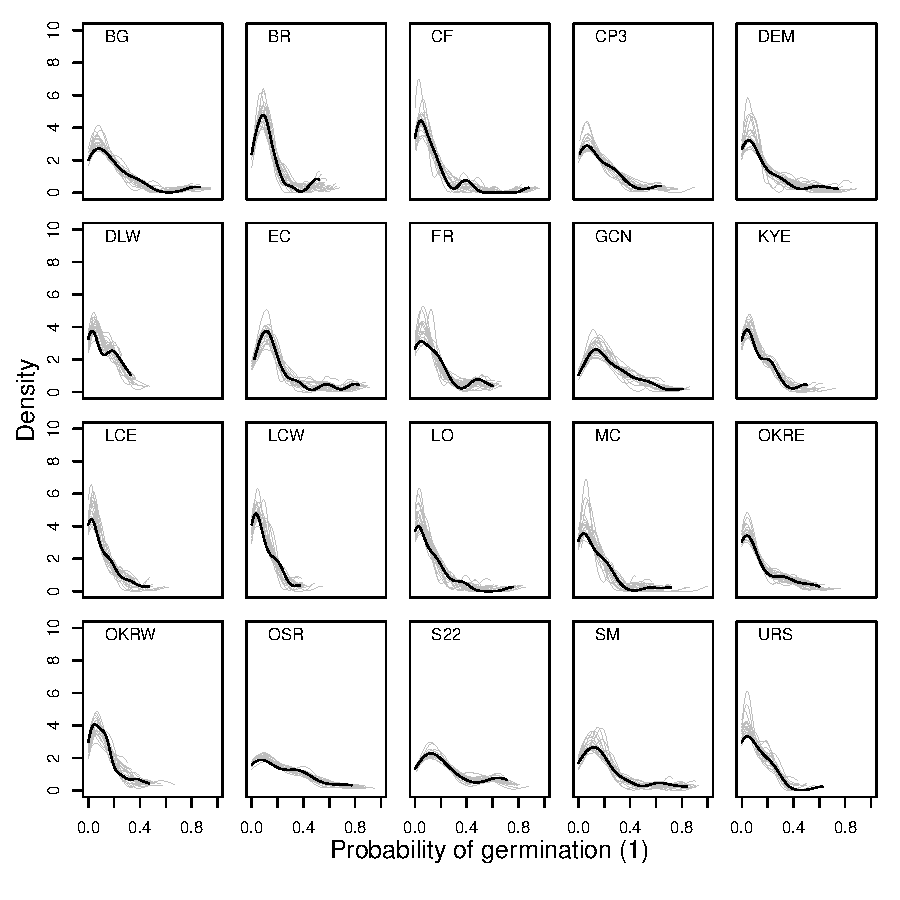
\includegraphics[page=1,width=1\textwidth]{../../figures/modelChecks/germination-population.pdf}  
 %   \caption{ }
 \label{fig:name}
\end{figure}

\begin{figure}[!h]
   \centering
       \includegraphics[page=2,width=1\textwidth]{../../figures/modelChecks/germination-population.pdf}  
 %   \caption{ }
 \label{fig:name}
\end{figure}

\begin{figure}[!h]
   \centering
       \includegraphics[page=3,width=1\textwidth]{../../figures/modelChecks/germination-population.pdf}  
 %   \caption{ }
 \label{fig:name}
\end{figure}

\begin{figure}[!h]
   \centering
       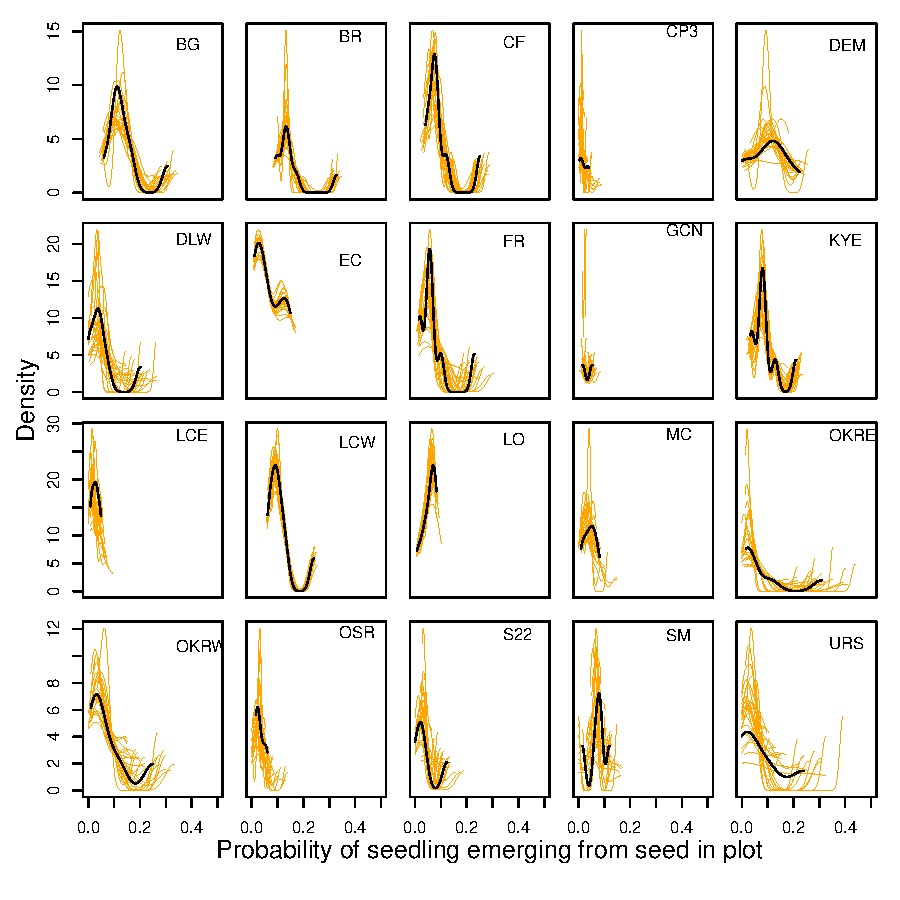
\includegraphics[page=1,width=1\textwidth]{../../figures/modelChecks/s0-population.pdf}  
 %   \caption{ }
 \label{fig:name}
\end{figure}



\clearpage
\newpage

Posterior predictive checks suggest that the model for the seed bag burial experiment adequately fit the data for germination. The majority (\hl{quantify}) of Bayesian p-values fell in the middle of the range $[0,1]$. The exception was the test static for the minimum probability of germination; the p-value for this test statistic was 1 in all populations and ages except for 2 instances. To explore this further, we examined the distribution of the minimum value of our simulated datasets, plotting these as histograms and overlaying the minimum of the observed dataset. This indicated that the extreme values of the test statistic are the result of the minimum value being the same in almost all simulated datasets and the observed dataset, which happens when we both observed 0 germinants and simulate 0 germinants.

\begin{figure}[!h]
   \centering
       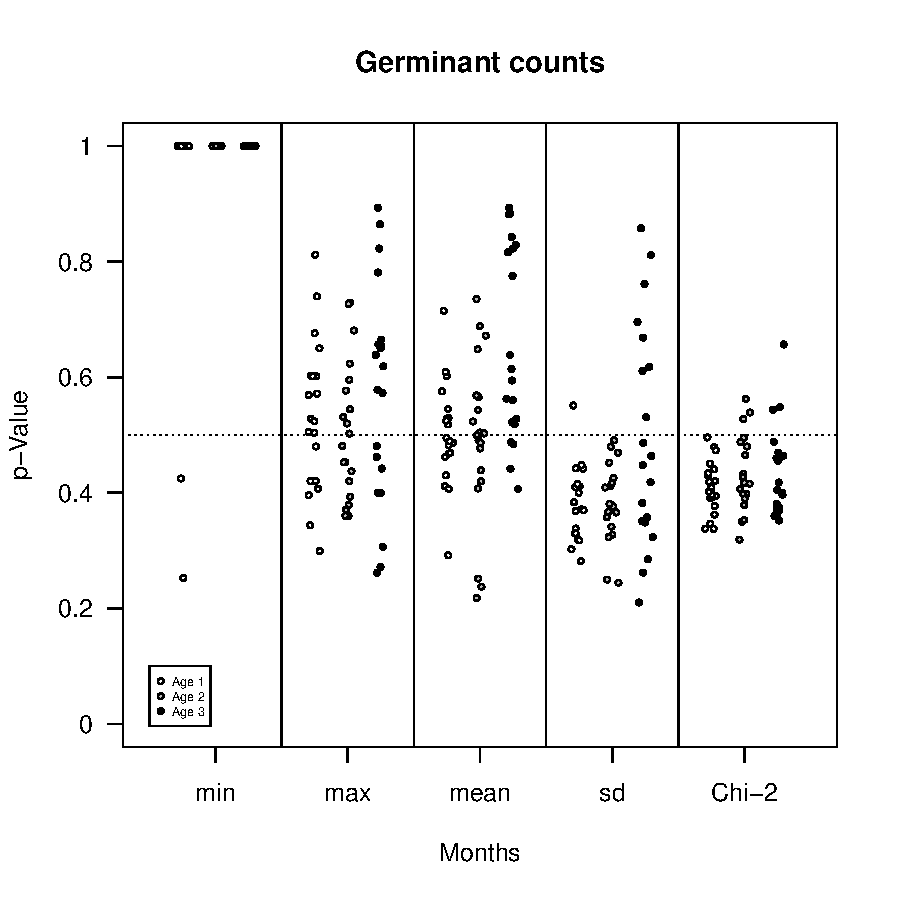
\includegraphics[page=1,scale=.5]{../../figures/modelChecks/germination-ppc.pdf}  
       \includegraphics[page=2,scale=.5]{../../figures/modelChecks/germination-ppc.pdf}  
 %   \caption{ }
 \label{fig:name}
\end{figure}

Posterior predictive checks also indicate that the model for the seed bag burial experiment adequately fit the data for counts of intact seeds. The majority of (\hl{quantify}) Bayesian p-values fell in the middle of the range $[0,1]$. There were several populations for which the p-value for the minimum probability of being an intact seed was 1. This occurred for seed counts in October of the second and third year. Histograms of the distribution of our simulated dataset (\hl{not shown}) indicate that the extreme values of the test statistic were calculated because the minimum of the observed data was 0 in those cases, and the majority of simulated datasets included 0 as a minimum. The distribution of p-values for the maximum in the first January also suggested possible lack of fit; examining the histograms for this test statistic indicated the lack of fit resulted in part because some populations had maximum probabilities of 1, which were adequately simulated by the model (e.g. population BR). The model also underestimated the maximum probability of success for some populations (e.g. populations BG, FR); however, this might be happening because the probability of all seeds remaining intact occurred in a limited number of bags and information from other bags pulls the probability of success away from high values. 

\begin{figure}[!h]
   \centering
       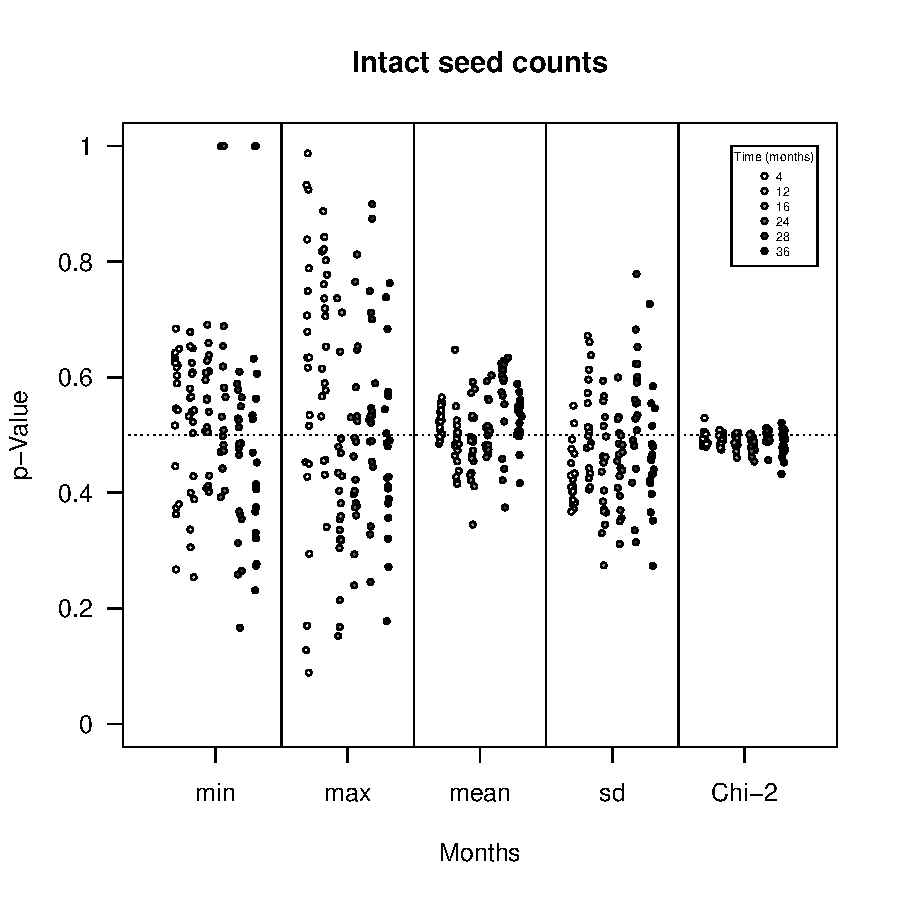
\includegraphics[page=1,scale=.5]{../../figures/modelChecks/decay-ppc.pdf}  
       \includegraphics[page=2,scale=.5]{../../figures/modelChecks/decay-ppc.pdf}  
 %   \caption{ }
 \label{fig:name}
\end{figure}

Finally, we also conducted posterior predictive checks for the number of seedlings emerging from plots. While individual simulations from the joint posterior were more idiosyncratic than the observed data, the test statistics generally support that the model for seedling emergence captures key characteristics such as the mean and standard deviation at the level of transects. Because we summed across plots to obtain the number of seeds produced and seedlings emerging in a transect, we had relatively few samples for fitting this model. We also lacked data to evaluate model fit in the first year for populations GCN and S22, as we did not observe any fruiting plants in plots at those population in 2007 (the year before the first year we observed seedling emergence). We again observed some lack of fit for the minimum probability of seedling emergence; we could attribute this to the minimum of the observed and simulated distribution both equaling zero. Lack of fit in $\chi^2$ was observed in the same populations in which we did not have data to evaluate test statistics, but was calculated as a p-value of 1 because we calculated this statistic internally in JAGS.

\begin{figure}[!h]
   \centering
       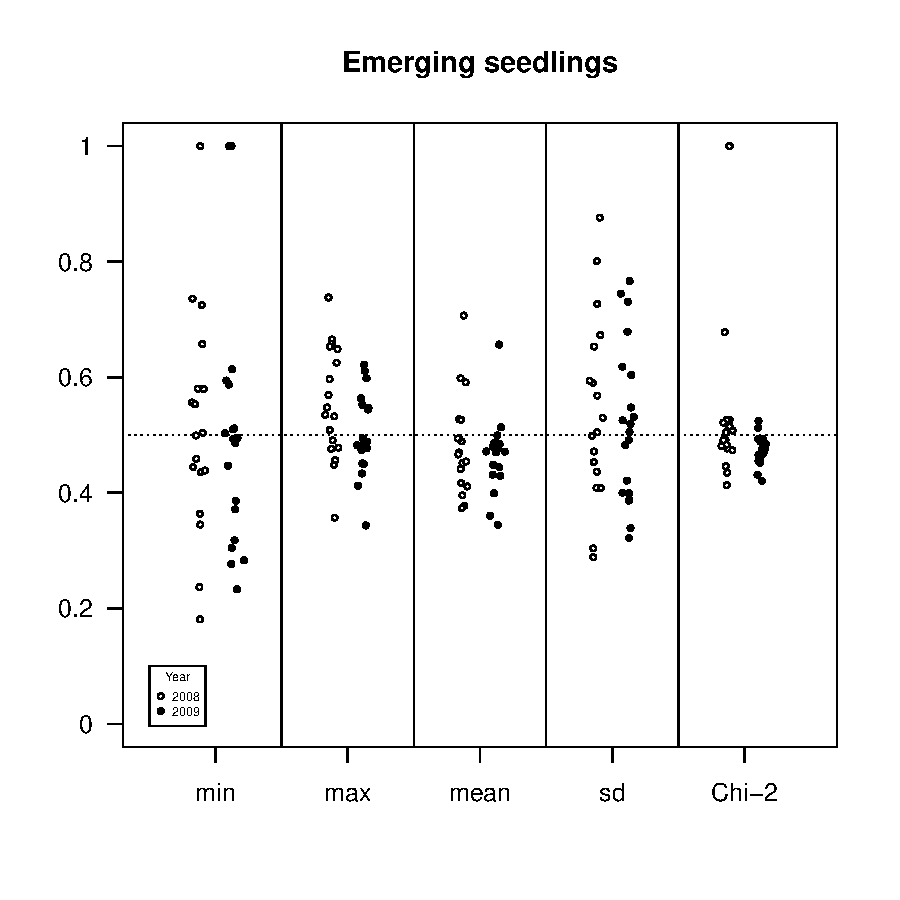
\includegraphics[page=1,scale=.75]{../../figures/modelChecks/s0-ppc.pdf}  
 %   \caption{ }
 \label{fig:name}
\end{figure}

\subsection{Seedling survival to fruiting}

For the model of seedling survival to fruiting, we simulated replicate binomial trials for each plot in each year at each site. The simulations calculate the population- and year-specific probability of survival from the model's joint posterior, and take the observed number of seedlings in a plot as the number of trials to simulate numbers of fruiting plants. 

We calculated the following test statistics for seedling survival to fruiting: minimum, maximum, mean, standard deviation, and $\chi^2$ values (\hl{these are recommended for binomial trials - find ref in Gelman - and Chi-2 as an omnibus statistic in Conn 2018}). We summarized the Bayesian p-values from these test statistics for each year as boxplots to represent the distribution of p-values across populations. The minimum of the observed versus simulated data proved to be extreme in all cases, as all simulated datasets and observations included 0 as a minimum. When examining the p-values of all other test statistics for population-and-year level fits, we noticed that the model performed adequately from 2006-2012 and 2017-2019; p-values for the mean, standard deviation and $\chi^2$ were ~0.5 in these years. However, test statistics were more extreme in 2013-2016, generally overestimating the number of fruiting plants. 

\begin{figure}[!h]
   \centering
       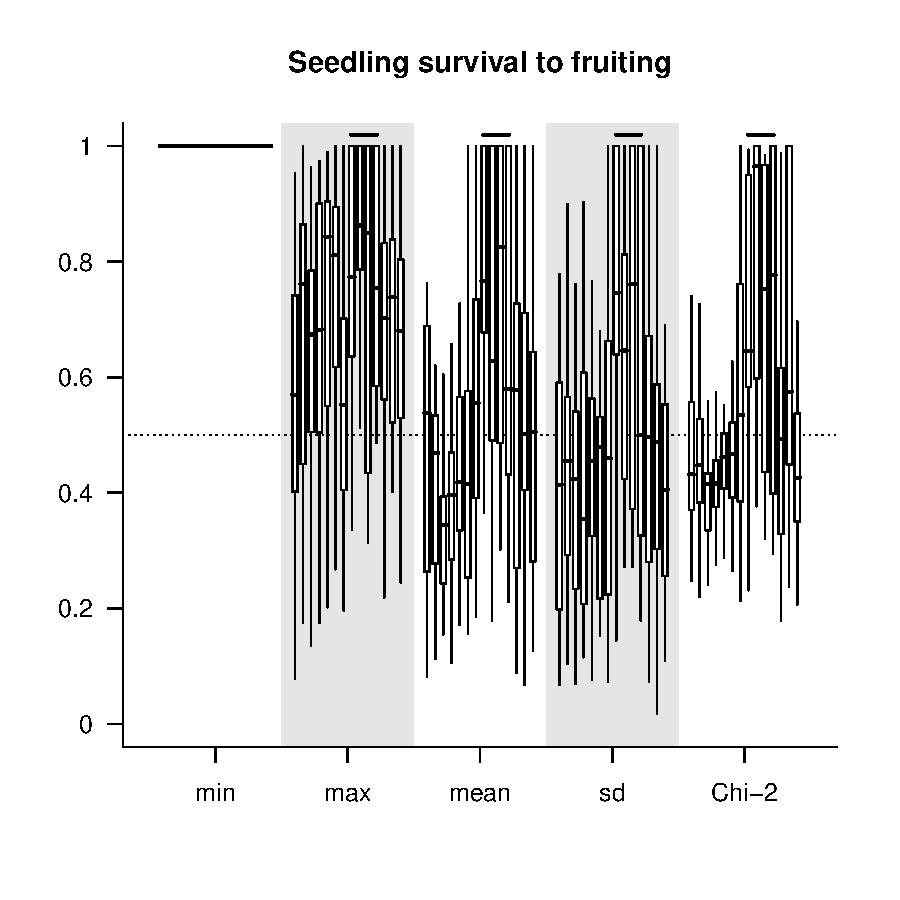
\includegraphics[page=1,width=1\textwidth]{../../figures/modelChecks/seedlingSurvival-pvals.pdf}  
    \caption{ Distribution of Bayesian p-values.  }
 \label{fig:name}
\end{figure}

We examined simulations from the model to further explore the issue of lack of fit. In years with relatively better model fit, we also had greater number of observations against which to compare our simulations. When there were few (0 or 1) plots with seedlings, test statistics tended to be high. The population-level estimate of seedling survival had a stronger effect in years with few seedlings; this likely pulled the year-level estimate towards the population-level mean. In other words, these are years in which there was stronger shrinkage.

\begin{figure}[!h]
   \centering
       \includegraphics[page=3,scale=.5]{../../figures/modelChecks/seedlingSurvival-ppc-population.pdf}  
       \includegraphics[page=11,scale=.5]{../../figures/modelChecks/seedlingSurvival-ppc-population.pdf}  
    \caption{ Two examples of years with more adequate (2008) and less adequate (2016) model fit. Patterns are similar across populations in other years (not shown). }
 \label{fig:name}
\end{figure}

We further examined the less adequate model fit by exploring correlates of the Bayesian p-values for $\chi^2$ values. Specifically, we found that the model for seedling survival to fruiting overestimated fruiting plant numbers when there were few or no seedlings in any plots. In some cases this may be because observed survival is 0 when there are few seedlings (trials) and zero fruiting plants (successes). With few seedlings, partial pooling would pull the estimated mean survival probability away from 0 and lead to overestimation. We also found that pooling may be a factor leading to overestimates if only a few plots contribute to the survival estimate in a given year. The checks thus suggest that the model overestimates seedling survival to fruiting in some years where observed survival is 0, either because of few seedlings and/or few plots with seedlings

\begin{figure}[!h]
   \centering
       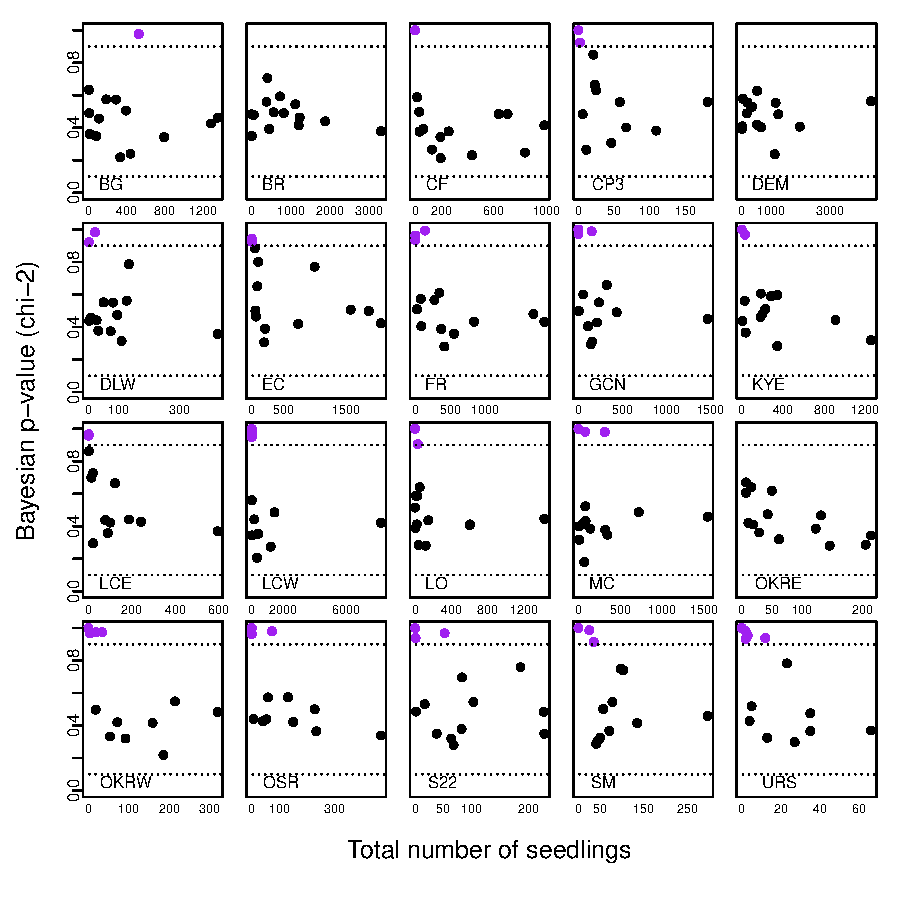
\includegraphics[page=1,width=.45\textwidth]{../../figures/modelChecks/seedlingSurvivalFruiting-populationyear.pdf}  
       \includegraphics[page=2,width=.45\textwidth]{../../figures/modelChecks/seedlingSurvivalFruiting-populationyear.pdf}  
    \caption{ (A) p-values for the $\chi^2$ of the number of fruiting plants at the population-and-year level plotted against the number of plots with nonzero numbers of fruiting plants. (B) p-values for the $\chi^2$ of the number of fruiting plants at the population-and-year level plotted against the total number of seedlings observed across all plots.  }
 \label{fig:name}
\end{figure}

The formula for calculating Bayesian p-values always handles ties (observed and simulated test statistic are equal) in the same way, so the p-value for cases where plots had 0 trials (and thus automatically 0 successes) is 1. Because our dataset includes years in which no plots at a site had any seedlings, this would show up as a poor model fit. Instead, we consider the absence of observed data to compare against as something that limits our ability to perform a model check rather than an indicator of poor fit. We thus recalculated p-values by excluding plots with 0 trials; the idea is similar to excluding ties from a sign test (as in \hl{Dixon, W.J. and Massey, F.J.Jr. (1951). An Introduction to Statistical Analysis. New York: McGraw-Hill.}.

\begin{figure}[!h]
   \centering
       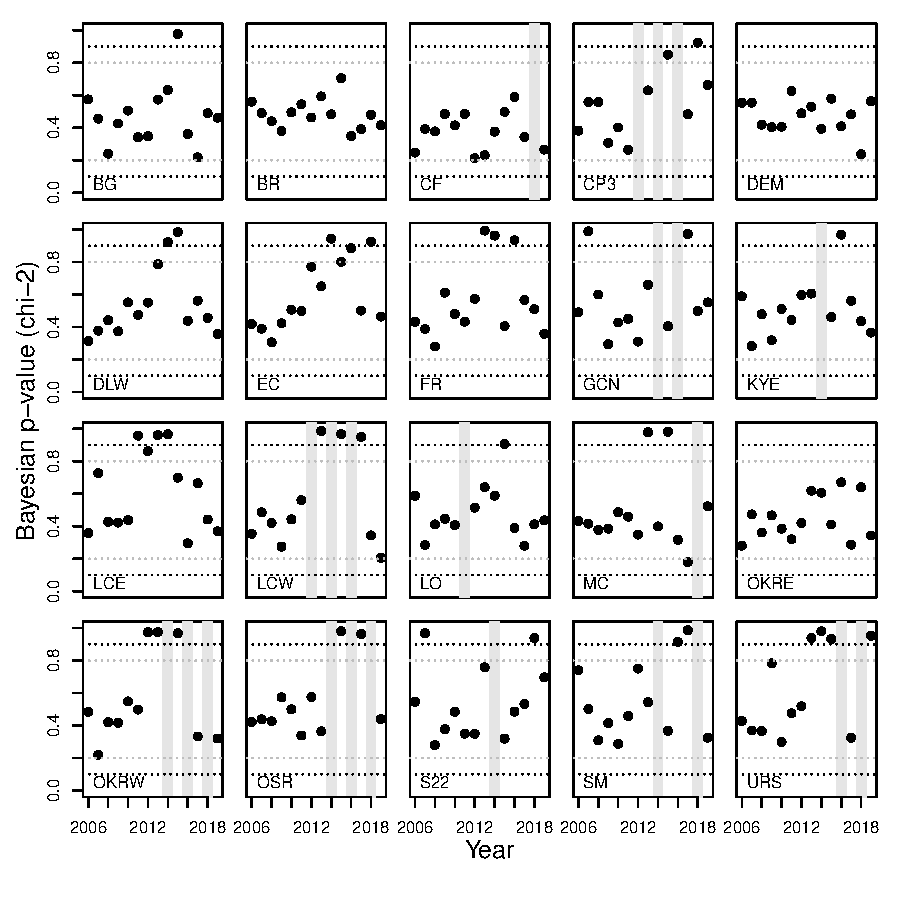
\includegraphics[page=1,width=\textwidth]{../../figures/modelChecks/seedlingSurvivalFruiting-zerotrials.pdf}  
    \caption{ p-values for the $\chi^2$ of the number of fruiting plants at the population-and-year level. Gray bars indicate years in which there were no plots with seedlings.  }
 \label{fig:name}
\end{figure}

\subsection{Fruits per plant}

Simulations: show distribution of fruit per plants per year*population (perhaps 1 representative year?)
PPC: show the similar estimates as for the belowground checks

\subsection{Seeds per fruit}







Because we were interested in whether the model accurately represented the age-specific and year-specific parameter means (this is the variation over time and age that is incorporated in a Leslie matrix representation of the system), we summarized the mean and median rate for each parameter. We also examined the standard deviation/coefficient of variation to diagnose whether the model represents variation about the mean. This is useful to help assess whether the confidence intervals placed on population growth rate are likely to be accurate. These are relatively generic summary statistics and the literature on posterior predictive checks identifies other kinds of statistics that could be used. However, these statistics correspond to key quantities that are used in subsequent steps beyond model fitting. 

Figure S4.1: summarize distribution of parameter specific p-values for mean, median, and CV
Figure S4.2: show summary distribution for different parameters vs. mean of parameter
Figure S4.3: for parameters (sigma, phi, F), show p-value plotted against observation year to diagnose the years in which the model may under/overestimate demographic parameters

\clearpage
\bibliography{/Users/gregor/Dropbox/bibliography/seeds}

\end{document}